% ============================ LAMPIRAN ============================
\lampiran{1}{Contoh kata pengantar}
\begin{tengah}
\textbf{KATA PENGANTAR}
\end{tengah}

Puji syukur penulis panjatkan kepada Allah Yang Maha Kuasa, sehingga dapat menyelesaikan penulisan skripsi ini. Untuk itu penulis juga sangat berterima kasih kepada yang terhormat:
\begin{enumerate}
\item Nama Pembimbing 1, selaku Pembimbing Utama dan Nama Pembimbing 2, selaku Pembimbing Pendamping atas saran dan bimbingannya.
\item Nama Dekan Fakultas Teknik, selaku Dekan Fakultas Teknik Universitas Muhammadiyah Buton.
\item Nama Ketua Program Studi, selaku Ketua Program Studi yang telah banyak membina kelancaran proses studi.
\item Nama Penguji 1 dan Nama Penguji 2, selaku penguji atas masukan dan saran selama Ujian Sarjana.
\item Penulis juga menyampaikan terima kasih kepada ………… (pihak terkait yang mendukung penyelesaian skripsi).
\end{enumerate}

\begin{kanan}
Baubau, November 2015

(Penulis)
\end{kanan}

\lampiran{2}{Contoh penulisan gambar dan tabel}
\textit{LVDT} ditempatkan pada puncak kolom, tengah kolom dan bawah kolom yang dimaksudkan sebagai data pengontrol nantinya dalam pengolahan hasil pengujian. Dua buah \textit{LVDT} juga ditempatkan pada balok untuk melihat \textit{displacement} yang terjadi pada daerah \textit{grouting}.

\begin{figure}[H]
\centering
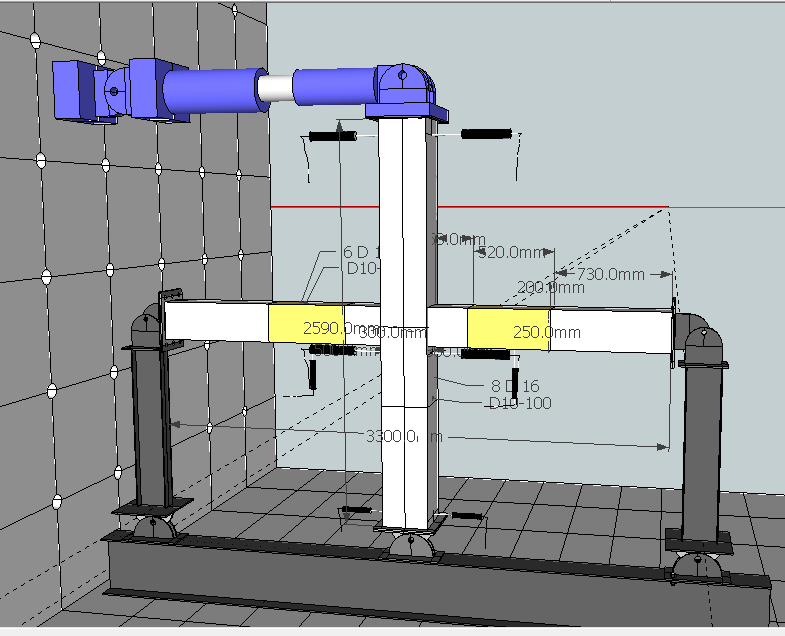
\includegraphics[width=0.5\textwidth]{../gambar/contoh-lvdt.png}
\caption{Detail penempatan \textit{LVDT}}
\end{figure}

\needspace{9cm}
Tabel L2.1 di bawah ini menyajikan resume data benda uji, termasuk di dalamnya ukuran penampang balok-kolom dan properti material penyusun yang nantinya merupakan dasar dalam pengolahan hasil pengujian.

\begin{singlespace}
\setlength{\tabcolsep}{10pt}
\begin{longtable}{|p{0.34\linewidth}|c|c|c|}
\caption{Resume data benda uji}\\
\hline
\textbf{Deskripsi} & \textbf{Balok} & \textbf{Kolom} & \textbf{\textit{Grouting}} \\
\hline
Panjang (L) & 3300 mm & 2950 mm & 520 mm \\
\hline
Tinggi (h) & 250 mm & 300 mm & 250 mm \\
\hline
Lebar (b) & 200 mm & 300 mm & 200 mm \\
\hline
Selimut (d) & 40 mm & 40 mm & 40 mm \\
\hline
f’c & 25 MPa & 25 MPa & 50 MPa \\
\hline
Diameter tulangan utama & 13 mm & 16 mm & 13 mm \\
\hline
Fy tulangan utama & 300 MPa & 300 MPa & 300 MPa \\
\hline
Diameter sengkang & 10 mm & 10 mm & 10 mm \\
\hline
Fy tulangan sengkang & 400 MPa & 400 MPa & 400 MPa \\
\hline

\end{longtable}
\end{singlespace}

\lampiran{3}{Contoh daftar tabel}
\begin{tengah}
\textbf{DAFTAR TABEL}
\end{tengah}
\begin{tanpagaris}
\begin{longtable}{@{}p{0.13\linewidth}p{0.67\linewidth}r@{}}
\textbf{Nomor} & \textbf{Judul} & \textbf{Halaman} \\
1 & Resume data benda uji & 2 \\
\end{longtable}
\end{tanpagaris}

\lampiran{4}{Contoh daftar gambar}
\begin{tengah}
\textbf{DAFTAR GAMBAR}
\end{tengah}
\begin{tanpagaris}
\begin{longtable}{@{}p{0.13\linewidth}p{0.67\linewidth}r@{}}
\textbf{Nomor} & \textbf{Judul} & \textbf{Halaman} \\
1 & Beberapa pola kurva histeresis & 5 \\
2 & Mekanisme plastifikasi rangka & 9 \\
\end{longtable}
\end{tanpagaris}

\lampiran{5}{Contoh daftar lampiran}
\begin{tengah}
\textbf{DAFTAR LAMPIRAN}
\end{tengah}
\begin{tanpagaris}
\begin{longtable}{@{}p{0.13\linewidth}p{0.67\linewidth}r@{}}
\textbf{Nomor} & \textbf{Judul} & \textbf{Halaman} \\
1 & Proses perakitan besi & 63 \\
2 & Proses pembuatan bekisting & 63 \\
3 & Pemasangan \textit{strain gauge} setelah pengelasan & 64 \\
4 & Persiapan pengecoran & 65 \\
5 & Proses pengecoran & 65 \\
6 & Pekerjaan persiapan tiang \textit{support} & 66 \\
7 & Tulangan yang akan di-\textit{grouting} & 66 \\
8 & Proses persiapan benda uji untuk melakukan \textit{grouting} pada sambungan & 67 \\
9 & Detail tulangan pada daerah \textit{grouting} & 67 \\
10 & Permukaan beton yang akan di-\textit{grouting}, dibersihkan kemudian dilapisi dengan \textit{epoxy} & 68 \\
11 & Proses \textit{grouting} & 68 \\
12 & Proses pengujian benda uji konvensional & 69 \\
13 & Proses pengujian benda uji \textit{grouting} & 69 \\
14 & Proses pengujian benda uji konvensional & 70 \\
15 & Kerusakan pada benda uji \textit{grouting} & 70 \\
\end{longtable}
\end{tanpagaris}

\lampiran{6}{Contoh daftar pustaka (gaya APA edisi ke-7)}
Tabel L6.1 merangkum pola penulisan daftar pustaka untuk berbagai jenis sumber. Sumber yang isinya dapat berubah (laporan daring, artikel daring, repositori kode) diakhiri tanggal akses dengan bentuk \textit{Diakses pada tanggal bulan tahun, dari alamat URL}.

\begin{singlespace}
\begin{longtable}{|p{0.24\linewidth}|p{0.68\linewidth}|}
\caption{Pola penulisan daftar pustaka menurut jenis sumber}\\
\hline
\textbf{Jenis sumber} & \textbf{Pola penulisan} \\
\hline
Buku & Penulis, A. B. (Tahun). \textit{Judul buku}. Penerbit. \\
\hline
Buku terjemahan & Penulis, A. B. (Tahun). \textit{Judul buku} (C. Penerjemah, Penerj.). Penerbit. \\
\hline
Bab dalam buku suntingan & Penulis, A. B. (Tahun). Judul bab. Dalam C. Editor (Ed.), \textit{Judul buku} (hlm. 10--25). Penerbit. \\
\hline
Artikel jurnal & Penulis, A. B. (Tahun). Judul artikel. \textit{Nama Jurnal, volume}(nomor), halaman awal--akhir. URL DOI \\
\hline
Prosiding & Penulis, A. B. (Tahun). Judul makalah. \textit{Nama Prosiding}, halaman awal--akhir. \\
\hline
Skripsi atau tesis & Penulis, A. B. (Tahun). \textit{Judul skripsi} [Skripsi, Nama Universitas]. Repositori. URL \\
\hline
Laporan lembaga & Nama Lembaga. (Tahun). \textit{Judul laporan}. Penerbit. \\
\hline
Laporan daring & Nama Lembaga. (Tahun). \textit{Judul laporan} [Laporan]. Diakses pada tanggal bulan tahun, dari URL \\
\hline
Lembar data (\textit{datasheet}) & Produsen. (Tahun). \textit{Judul lembar data} (Versi x) [Lembar data]. URL \\
\hline
Artikel berita atau blog & Penulis, A. B. (Tahun, tanggal bulan). Judul artikel. \textit{Nama Situs}. Diakses pada tanggal bulan tahun, dari URL \\
\hline
Repositori kode & Penulis. (Tahun). \textit{Nama repositori} [Kode sumber]. GitHub. Diakses pada tanggal bulan tahun, dari URL \\
\hline
Tanpa penulis & \textit{Judul sumber}. (Tahun). Penerbit. \\
\hline
\end{longtable}
\end{singlespace}

\begin{tengah}
\textbf{DAFTAR PUSTAKA}
\end{tengah}
\begin{pustaka}
AlQahtani, S. A., \& Alhassany, M. (2013). Comparing different LTE scheduling schemes. \textit{2013 9th International Wireless Communications and Mobile Computing Conference (IWCMC)}, 264--269.

Andrews, M. (2007). A survey of scheduling theory in wireless data networks. \textit{Wireless Communications, 143}, 1--17.

Badan Pusat Statistik. (1997). \textit{Statistik Indonesia 1996}. Badan Pusat Statistik.

Capozzi, F., Piro, G., Grieco, L. A., Boggia, G., \& Camarda, P. (2013). Downlink packet scheduling in LTE cellular networks: Key design issues and a survey. \textit{IEEE Communications Surveys \& Tutorials, 15}(2), 678--700.

Espressif Systems. (2023). \textit{ESP32-WROOM-32 datasheet} (Versi 3.3) [Lembar data]. \url{https://www.espressif.com/en/support/documents/technical-documents}

Gaman, P. M., \& Sherrington, K. B. (1994). \textit{Ilmu pangan} (M. Gardjito, S. Naruki, Murdiati, \& Sardjono, Penerj.). Gadjah Mada University Press.

Ghosh, A., Zhang, J., Andrews, J. G., \& Muhamed, R. (2010). \textit{Fundamentals of LTE}. Prentice Hall.

Kementerian Komunikasi dan Digital. (2025). \textit{Judul laporan tahunan} [Laporan]. Diakses pada 21 Oktober 2026, dari \url{https://www.komdigi.go.id/contoh-laporan.pdf}

\textit{Panduan penulisan karya ilmiah}. (2020). Penerbit Universitas.

Penulis, A. (2020). Judul bab dalam buku suntingan. Dalam B. Editor \& C. Editor (Ed.), \textit{Judul buku suntingan} (hlm. 10--25). Penerbit.

Penulis, A. B. (2022). \textit{Judul skripsi atau tesis} [Skripsi, Universitas Muhammadiyah Buton]. Repositori Universitas Muhammadiyah Buton. \url{https://repository.example.ac.id/contoh}

Penulis, C. D. (2024). Judul artikel jurnal dengan DOI. \textit{Jurnal Teknologi dan Sistem Komputer, 12}(1), 45--58. \url{https://doi.org/10.xxxx/xxxxx}

Penulis, E. (2026, 5 Maret). Judul artikel berita atau blog. \textit{Nama Situs}. Diakses pada 21 Oktober 2026, dari \url{https://www.contoh.com/artikel}

Penulis, F. (2024). \textit{Nama repositori} [Kode sumber]. GitHub. Diakses pada 21 Oktober 2026, dari \url{https://github.com/pengguna/repositori}

Radiati, L. E. (2000). Penghambatan bakteri enteropatogen oleh ekstrak jahe. \textit{Jurnal Habitat, 12}(2), 81--91.

Xu, Y., \& Fischione, C. (2012). Real-time scheduling in LTE for smart grids. \textit{Proceedings of the 5th International Symposium on Communications, Control and Signal Processing}, 2--4.
\end{pustaka}

\lampiran{7}{Daftar periksa kelengkapan skripsi}
Gunakan daftar periksa pada Tabel L7.1 sebelum menyerahkan naskah kepada dosen pembimbing atau penguji.

\begin{singlespace}
\begin{longtable}{|p{0.06\linewidth}|p{0.66\linewidth}|p{0.16\linewidth}|}
\caption{Daftar periksa format dan kelengkapan skripsi}\\
\hline
\textbf{No} & \textbf{Hal yang diperiksa} & \textbf{Sudah} \\
\hline
1 & Kertas A4, margin kiri 4 cm, atas 4 cm, kanan 3 cm, bawah 3 cm; tidak ada teks, tabel, atau gambar yang melewati margin & \\
\hline
2 & Huruf Times New Roman 12 pt, 1,5 spasi, alinea menjorok 1 cm, rata kanan-kiri & \\
\hline
3 & Sampul, lembar persetujuan, pengesahan, dan pernyataan keaslian lengkap dan benar & \\
\hline
4 & Abstrak dan \textit{Abstract} maksimal 300 kata, satu paragraf, memuat kata kunci & \\
\hline
5 & Kata pengantar, daftar isi, daftar tabel, dan daftar gambar sudah diperbarui & \\
\hline
6 & Setiap bab dimulai di halaman baru; judul bab dan subbab sesuai format & \\
\hline
7 & Nomor halaman benar: romawi di bagian awal, awal bab di tengah bawah, halaman lain di kanan atas & \\
\hline
8 & Rumusan masalah, tujuan, dan kesimpulan saling sesuai & \\
\hline
9 & Penelitian terdahulu minimal empat dalam 10 tahun terakhir & \\
\hline
10 & Metode dapat diulangi orang lain (alat, bahan, prosedur, variabel jelas) & \\
\hline
11 & Tabel berbentuk kotak penuh, bernomor per bab, judul di atas, dan dirujuk di teks & \\
\hline
12 & Gambar jelas, bernomor per bab, judul di bawah, dan dirujuk di teks & \\
\hline
13 & Persamaan bernomor di kanan dan simbolnya dijelaskan & \\
\hline
14 & Semua sitasi di teks ada di daftar pustaka, dan sebaliknya & \\
\hline
15 & Daftar pustaka gaya APA, urut abjad, sumber web memuat tanggal akses & \\
\hline
16 & Bahasa baku, tidak memakai kata ganti orang pertama, istilah asing ditulis miring & \\
\hline
17 & Hasil pemeriksaan kemiripan (plagiasi) sudah dilampirkan & \\
\hline
18 & Persetujuan dosen pembimbing I dan II sudah diperoleh & \\
\hline
\end{longtable}
\end{singlespace}
